\documentclass[12pt]{article}

\usepackage[bottom = 15mm]{geometry}
\usepackage[utf8]{inputenc}
\usepackage[T2A]{fontenc}
\usepackage[russian]{babel}
\usepackage{graphicx}
\usepackage{caption}
\usepackage{amssymb, gensymb, amsmath}
\usepackage{mathrsfs}
\usepackage{array, colortbl}
\usepackage{multicol}


\textwidth = 16 cm
\textheight = 23  cm
\oddsidemargin = 0 pt
\topmargin = -1.5 cm
\parindent = 20 pt
\parskip = 0 pt
\flushbottom


\title{{\bf Задача 4.\,5.\,3 \\ Сканирующий интерферометр}}
\author{Лось Денис (группа 611)}
\date{11 апреля 2018}

\begin{document}

\maketitle

\paragraph{Цель работы: } знакомство с устройством и работой газового лазера непрерывного действия, со спектральными характеристиками лазерного излучения, а также с устройством и принципом действия сканирующего интерферометра Фабри - Перо; определение медмодового расстояния и приборной ширины отдельной моды излучения лазера, оценка газокинетической температуры в разряде, рассчёт дисперсионной области, разрешающей способности и коэффициента отражения зеркал сканирующего интерферметра.

\paragraph{В работе используются: } He-Ne-лазер с блоком питания, сканирующий интерферометр Фабри-Перо, поляроид, пластинка $\lambda / 4$, линза, фотодиод, электронный осциллограф.

\section*{Теоритическая часть: He-Ne-лазер}
\par
	Основным элементом гелий-неонового лазера непрерывного действия является газоразрядная трубка, которая заполнена смесью гелия и неона. Концы трубки закрыты плоскопараллельными стеклянными или кварцевыми пластинами $P_1$ и $P_2$, установленными под углом Брюстера к её оси. Соотвественно линейно поляризованный свет с электрическим вектором, лежащим в плоскости падения, не испытывает потерь на отражение, а следовательно, лазер генерирует линейно-поляризованное излучение. В загнутых концах трубки располагаются катод $K$ и анод $A$. Трубка помещена между зеркалами $S_1$ и $S_2$, образующими интерферометр Фабри-Перо, который в данном случае играет роль оптического резонатора.
\begin{figure}[h!]
	\centering
	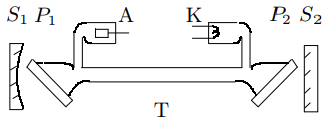
\includegraphics[width = 7cm, height = 3cm]{image1.png}
	\caption{Устройство гелий-неонового лазера}
\end{figure}
\par
	Так как рабочим газом лазера является неон, то для возбуждения лазерной генерации необходимо создать инверсную заселённость уровней рабочего перехода неона. Инверсная заселённость в данном лазере достигается главным образом из-за передачи возбуждения атомам неона от атомов гелия, которые возбуждаются  в разряде электронным ударом.
\par
	Активная среда, обладающая инверсной заселённостью уровней, способна усиливать оптическое излучение на частоте рабочего перехода, что происходит вследствие индуцированного когерентного излучения возбуждённых атомов под действием поля световой волны.
\par
	Если мы поместим кювету с активной средой между зеркалами интерферометра Фабри-Перо, то испущенный вдоль оси свет будет многократно отражаться, при этом будут обеспечиваться условие лазерной генерации света --- превышение усиления на потерями. Стоит отметить, что потери в гелий-неоновом лазере обусловлены главным образом неидеальным отражением от зеркал, т.е. уходом излучения из резонатора.
\par
	В интерферометрах Фабри-Перо, которые используются в лазерах,излучение распространяется вдоль оси интерферометра. Если на полном оптическом пути $2L$, где $L$ ---  расстояние между зеркалами, будет укладываться целое число длин волн, то наступит резонанс, а в интерферометре возникнет стоячая волна. Стоит отметить, что при этом волна дважды отражённая от зеркал, вернётся к испустившему её атому в той же фазе, в которой она была испущена. Условие резонанса:
\begin{equation}
	2L = m \lambda \quad (m \in \mathbb{Z}) \label{res}
\end{equation}
\par
	Различным значениям порядка $m$ соотвествуют стоячие волны разных частот, которые называют типами колебаний, или {\bf модами}. Выражение для междмодового расстояния $\Delta \nu$:
\begin{equation}
	\Delta \nu = \frac{c}{2L} \label{NU}
\end{equation}
	Стоит отметить, что есть так называемые {\bf продольные} и {\bf поперечные} моды. Продольные моды отличаются по частоте на величину $\Delta \nu$. Поперечные моды отличаются от продольных распределение интенсивности по сечению пучка. Их частоты отличаются от соответствующих частот продольных мод на величину, малую по сравнению с межмодовым расстоянием $\Delta \nu$.
\section*{Теоритеская часть: сканирующий интерферометр}
\par
	В данном случае мы рассмотрим сканирующий интерферометр, который представляет собой высокодобротный интеферометр Фабри-Перо с периодически изменяемой базой.
\begin{figure}[h!]
	\centering
	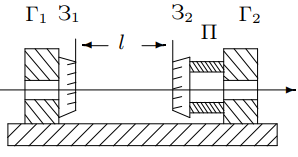
\includegraphics[width = 10cm, height = 4cm]{image2.png}
	\caption{Устройство сканирующего интерферометра}
\end{figure}
\par
	На жёстком массивном основании расположены две юстировочные головки $\text{Г1}$ и $\text{Г2}$, на которых укреплены зеркала $\text{З}_1$ и $\text{З}_2$. Зеркало $\text{З}_1$ установленно непосредственно на головке $\text{Г1}$, а зеркало $\text{З}_2$ связано с головкой $\text{Г2}$ через пьезокерамический элемент $\text{П}$. Пьезокерамический элемент П позволяет периодически изменять базу интерферометра на величину порядка длины световой волны. Если вдоль оси интерферометра распространяется световое излучение с длиной волны $\lambda$, то при выполнении условия аналогичного (\ref{res}) возникает резонанс
\begin{equation}
	2 l = m \lambda \quad (m \in \mathbb{Z}) \label{res2}
\end{equation}
\par
	Внешнее излучение с длиной волны, удовлетворяющей условию (\ref{res2}), полностью проходит через интерферометр. Если на интереферометр падает излучение с различными длинами волн, то одновременно может возникнуть несколько резонансо. Собственные моды интерферометра будут отличаться на
\[
	\Delta f = \frac{c}{2l}
\]
\par
	Величина $\Delta f$ называется {\bf дисперсионной областью} спектрального прибора. Можно также записать
\begin{equation}
	\Delta \lambda_\text{си} = \frac{\lambda}{m} = \frac{\lambda^2}{2l} \label{S}
\end{equation}
\par
	Разрешающая способность спектрального прибора
\[
	R = \frac{R}{\delta R},
\]
где $\delta R$ --- минимальная разность длин волн, разрешимая прибором вблизи длины волны $\lambda$. Для определения $\delta R$ обычно используют критерий разрешения Релея. Для разрешающей способности интереферометра Фабри-Перо можем записать
\begin{equation}
	R = \frac{2 \pi l}{\lambda \left(1 - r \right)}, \label{Re}
\end{equation}
где $r$ --- коэффициент отражения зеркал.
\par
	Выражение в единицах частоты
\[	
	\delta f = \nu \frac{\delta \lambda}{\lambda} = \frac{c}{2l} \frac{1-r}{\pi}
\]
\section*{Экспериментальная установка}
\par
	Рассмотрим конфигурацию экспериментальной установки, схема которой представлена на рис.3. Излучение гелий-неонового лазера проходит через поляризационную развязку Р и линзу Л и поступает на вход сканирующего интерферометра.
\begin{figure}[h!]
	\centering
	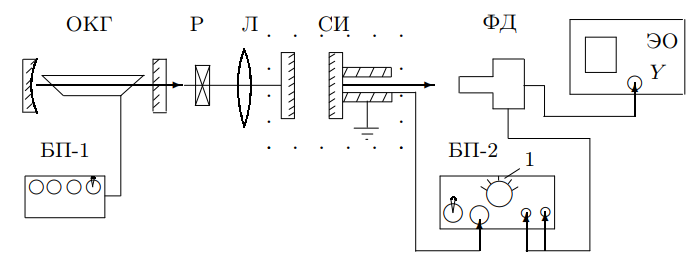
\includegraphics[width = 12cm, height = 5cm]{image3.png}
	\caption{Схема установки для исследования доплеровского контура излучения лазера}
\end{figure}
\par
	Поляризационная развязка предотвращает попадание в лазер излучения, отразившегося от элементов оптического тракта, которое может существенно повлиять на работу лазера. Развязка состоит из поляроида и пластинки $\lambda / 4$, главные направления которой установлены под углом $45 \degree$ по отношению к разрешённому напрвлению поляроида. После развязка П свет приобретает циркулярную поляризацию (например, по правому кругу). При отражении от передней поверхности линзы, от зеркада сканирующего интерферометра и т.п. свет распространяется в обратном направлении в виде левополяризованной волны. Такая волна, пройдя через пластинку $\lambda / 4$, вновь приобретает линейную поляризацию. Однако направление колебаний в этой волне оказывается перпендикулярным направлению разрешённых колебаний подяроида, поэтому до лазера отражённая волна не доходит.
\par
	Линза Л служит для уменьшения расходимости пучка, поступающего на вход сканирующего интерферометра. Линза снабжена поперечными и продольными салазками для юстировки прибора на максимум сигнала.
\par
	Излучение, прошедшее сквозь сканирующий интерферометр, поступает на фотодиод ФД. Напряжение с фотодиода через усилитель подаётся на вертикальный вход электронного осциллографа ЭО.	
\section*{Ход работы и полученные результаты}
\par
	Собрав экспериментальную установку, схема которой представлена на рис.3., и настроив систему, получим на осциллографе картину, где укладывается 1-2 доплеровских контура. Далее проведём рассчёты и некоторые измерения.
\begin{enumerate}
	\item
		В данной установке расстояние между зеркалами лазера $L = 65$ см. Длина волны лазера $\lambda = 632.8$ нм. Проблема здесь состоит в том, что мы не знаем точно, с какой погрешностью были определены эти величины. Однако рассчитаем межмодовое расстояние резонатора в единицах в единицах $\nu$ и $\lambda$, используя (\ref{NU}). Скорость света $c$ считаем равной $299792458$ $\text{м} \, / \, \text{c}$. 
		\begin{align*}
			\Delta \nu &= 231 \, \text{МГц} \\
			\Delta \lambda &= 309 \, \text{фм}
		\end{align*}
	\item
		Между модами на экране число промежутков $n = 3$. Оценим видимую ширину спектральной линии неона $\Delta \lambda (Ne)$:
		\[
			\Delta \lambda (Ne) = 1.0 \, \text{пм}
		\]
	\item
		Полагая, что ширина спектральной линии обусловлена эффектом Доплера и что видимая ширина линии неона порядка полуширины доплеровского контура ($\Delta \lambda(Ne) \approx \Delta \lambda_D$) оценим среднюю скорость атомов неона $v_x$ и газокинетическую  температуру $T$ в разряде:
	\[
		\frac{\Delta \lambda_D}{\lambda} \approx \frac{v_x}{c}; \qquad \frac{m v_x^2}{2} \approx \frac{kT}{2},
	\]
		где $v_x$ --- скорость молекул неона вдоль оси лазера; $m_\text{Ne} = 20.2$ а.е.м, $1 \, \text{а.е.м.} = 1.66 \cdot 10^{-24} \, \text{г}$.
		В результате получим, что
		\[
			v_x \approx 474 \, \frac{\text{м}}{\text{с}}; \qquad T \approx 546 \, \text{K}
		\] 
	\item
		Рассчитаем дисперсионную область $\Delta \lambda_\text{си}$ сканирующего интерферометра по формуле (\ref{S}). В данной установке $l = 9$ см.
		\[
			\Delta \lambda_\text{си} = 2.2 \, \text{пм}
		\]
		Заметим, что $\Delta \lambda_\text{си} \approx 2 \cdot \Delta \lambda (Ne) = \Delta \lambda_\text{неон}$
	\item
		Определим ширину отдельной моды на полувысоте по сравнению с межмодовым расстоянием $\Delta \lambda$. Получим, что $\delta \lambda \approx 0.2 \lambda$. В результате оценим разрешаюшую способность $R$
		\[
			R \approx 10^7
		\]
	\item
		Оценим коэффициент отражения зеркал интерферометра $r$ по формуле (\ref{Re})
		\[
			r = 1 - \frac{2 \pi l}{\lambda R} \approx 0.91
		\]
	\item
		Приведём изображение одной из наблюдаемых картин
		\begin{figure}[h!]
			\centering
			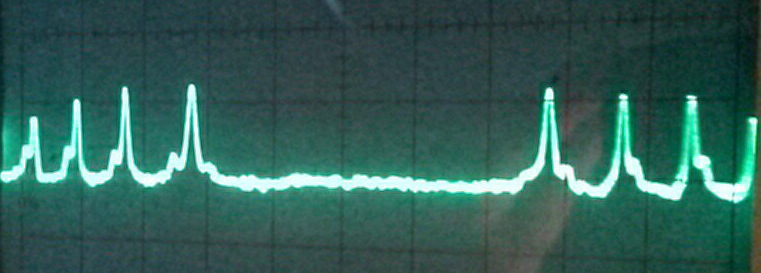
\includegraphics[width = 11cm, height = 4cm]{image4.png}
			\caption{Одна из картин, наблюдаемых на экране осциллографа}
		\end{figure}
\end{enumerate}
\section*{Выводы}
\par
	В результате работы мы определили межмодовое расстояние, оценили газокинетическую температуру в разряде, а также среднюю скорость атомов неона. Мы также оценили дисперсионную область сканирующего интерферометра и сравнили её с $\Delta \lambda_\text{неон}$. Сравнив ширину отдельной моды на полувысоте с межмодовым расстоянием, мы оценили разрешающую способность $R$, а также коэффициент отражения зеркал интерферометра $r$.
\par
	Произведённые оценки соответсвуют предполагаемым эталонным ожидаемым значениям (кроме $r$), приведённым в описании к работе. Однако стоит отметить, что кроме того, что нам не были известны погрешности, с которыми были определены параметры установки, непосредственные оценки величин, которые мы делали, анализируя изображение на экране осциллографа (к примеру, для оценки $r$), также не позволяют говорить о своей высокой точности, но так как в данной работе ключевым моментом является как раз то, что мы лишь должны были произвести оценку необходимых величин, то полученные результаты являются вполне приемлемыми.
\par
	Небольшую, но всё же сложность, составили также настройка и центровка системы во время сборки экспериментальной установки.
\end{document}